\documentclass[12pt]{article}

\usepackage{vmargin}
\usepackage{setspace}
\usepackage[ruled, linesnumbered, french, onelanguage]{algorithm2e}
\usepackage{amsmath, amsthm, amssymb, amsfonts}
\usepackage{enumitem}
\usepackage[utf8]{inputenc}
\usepackage{hyperref}
\usepackage{graphicx}
\usepackage{float} % here for H placement parameter
\graphicspath{{figures/}}

\setlength{\parindent}{0pt}

\title{Devoir 2}
\author{Jérémy Bouchard}
\date{\today}

\begin{document}

\begin{titlepage}
	\doublespacing
	\centering
	
	UNIVERSITÉ DU QUÉBEC À CHICOUTIMI \\
	
	\vspace{4.7cm}
	
	DEVOIR 2 \\
	
	\vspace{4.7cm}
	
	PAR \\
	JÉRÉMY BOUCHARD (BOUJ08019605) \\
	JEAN-PHILIPPE SAVARD (SAVJ04079609) \\
	ALEXIS VALOTAIRE (VALA09129509) \\
	
	\vspace{4.7cm}
	
	DEVOIR PRÉSENTÉ À \\
	M. FRANÇOIS LEMIEUX \\
	DANS LE CADRE DU COURS D'ALGORITHMIQUE (8INF433)
\end{titlepage}

\newpage

\textit{Note :} Le code source \LaTeX \:est disponible à l'URL suivant : \\ 
\url{https://github.com/AlexisCode101/algo-devoir-2}

\newpage

\onehalfspacing

\section*{Question 1}
Le théorème sur les récurrences que nous avons vu en classe possède
une version plus simple dans le cas où la fonction f(n) est un polynôme.
Lorsque la récurrence est de la forme:
\begin{align*}
	T(n) = aT\Big(\frac{n}{b} + cn^k\Big)
\end{align*}

où c et k sont des constantes réelles positives, alors la solution est
donnée par:

\[T(n) \begin{cases} 
      \Theta\big(n^{log_ba}\big) & \text{si } a>b^k \\
      \Theta\big(n^klg \: n\big) & \text{si } a=b^k \\
      \Theta\big(n^k\big) & \text{si } a<b^k
   \end{cases}
\]	

Nous avons vu en classe la démonstration du premier cas (où  \(a > b^k\)
).
Utilisez le théorème sur les récurrences vu en classe pour démontrer les
deux autres cas.


\newpage

\section*{Question 2}
L’algorithme de Dijkstra que nous avons vu en classe, nous permet
d’obtenir la longueur du plus court chemin entre un noeud source et
tous les autres noeuds mais il ne donne pas les chemins eux-mêmes. Comment modifieriez-vous cet algorithme afin d’obtenir cette information? Notez que la modification est mineure si vous choisissez la bonne façon de représenter les chemins.

\newpage

\section*{Question 3}
Considérez le graphe dirigé de la figure suivante:

\begin{figure}[H]
	\centering
	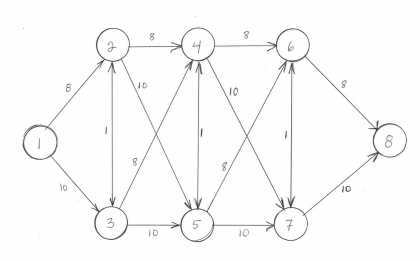
\includegraphics[width=12cm]{q3} 
\end{figure}

Montrez le contenu du tableau \(D\), de l’ensemble \(S\) ainsi que la valeur de la variable \(v\) après chacune des itérations de l’algorithme. Décrivez toutes les étapes de l’algorithme Dijkstra. Utilisez le noeud 1 comme source.

\newpage

\section*{Question 4}
Résoudre les récurrences suivantes. \\

\textbf{a) } \(T(n)=2T\big(\frac{n}{2}\big)+1\) \\

\textbf{b) } \(T(n)=T\big(\frac{9n}{10}\big)+n\) \\

\textbf{c) } \(T(n)=16T\big(\frac{n}{4}\big)+n^2\) \\

\textbf{d) } \(T(n)=7T\big(\frac{n}{3}\big)+n^2\) \\

\textbf{e) } \(T(n)=7T\big(\frac{n}{2}\big)+n^2\) \\

\textbf{f) } \(T(n)=2T\big(\frac{n}{4}\big)+\sqrt{n}\) \\

\textbf{g) } \(T(n)=3T\big(\frac{n}{2}\big)+5n\) \\

\textbf{h) } \(T(n)=T\big(\frac{n}{2}+5\big)+1\) \\

\newpage

\section*{Question 5}
Considérez la matrice suivante
\begin{align*}
	F = 
	\begin{pmatrix}
		0 & 1 \\
		1 & 1 
	\end{pmatrix}
\end{align*}

Soit \(i\) et \(j\), deux entiers. Quel est le produit du vecteur (\(i\), \(j\)) et de la matrice \(F\)? Qu’arrive-t-il si i et j sont deux nombres consécutifs de la suite de Fibonacci? Utilisez cette idée pour concevoir un algorithme diviser-pour-régner capable de calculer le nième nombre de Fibonacci en temps \(\Theta (log \: n)\) en considérant (faussement) que les multiplications
prennent un temps constant. Expliquez le lien entre votre algorithme et l’algorithme fib3 du devoir 1.

\newpage

\section*{Question 6}
Soit \(X[1 \dots n]\) et \(Y [1 \dots n]\) deux tableaux, chacun contenant \(n\) nombres déjà triés. Donnez un algorithme diviser-pour-régner pour trouver le médian des \(2n\) éléments présents dans les tableaux \(X\) et \(Y\). Le temps d’exécution de votre algorithme doit être dans \(\Theta (log \: n)\) en pire cas.

\end{document}
